% !TeX root = ../Skript_DB.tex
\cohead{\Large\textbf{Optimieren}}
\subsection[Optimierung]{Optimierung von Datenbanken}
Bisher wurde jeder Entitätstyp und jede Beziehung als eigene Tabelle auf der Datenbank dargestellt. Für alle Beziehungen, die von der Kardinalität 1:X oder X:1 sind, kann man die Informationen der Beziehungstabelle in die Tabelle eines der beiden Entitätstypen verschieben.
\begin{tcolorbox}[title=Optimierung]
	Für 1:X oder X:1 Beziehungen kann die Beziehungstabelle in einer der Entitätstyp-Tabellen integriert werden, indem man den Primärschlüssel des einen Entitätstyps in die Tabelle des anderen Entitätstyps als Fremdschlüssel hinzufügt.
\end{tcolorbox}
Betrachten wir folgendes Beispiel:
\begin{minipage}{\textwidth}
	\centering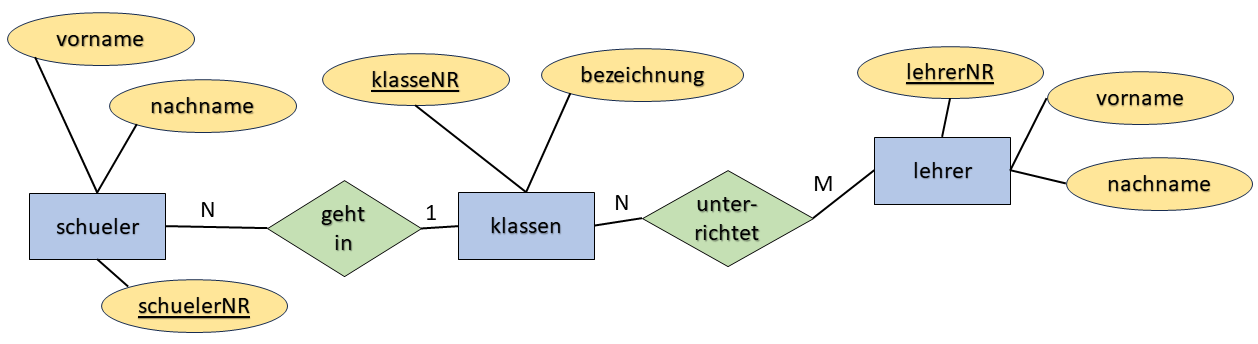
\includegraphics[width=\textwidth]{\pics/Optimierung.png}
\end{minipage}

Bildet man jeden Entitätstyp und jede Beziehung als eine eigene Tabelle ab, so erhält man z.B.:
\begin{minipage}{\textwidth}
	\begin{minipage}{0.5\textwidth}
		\begin{tabular}{lll}
			\multicolumn{3}{c}{\lstinline!schueler!}\\
			\hline
			\underline{\lstinline!schuelerNR!}&\lstinline!vorname!&\lstinline!nachname!\\
			\hline
			105&Max&Verstappen\\
			106&Charles&Leclerc\\
			110&Lewis&Hamilton\\
		\end{tabular}
	\end{minipage}%
	\begin{minipage}{0.5\textwidth}
		\begin{tabular}{ll}
			\multicolumn{2}{c}{\lstinline!klasse!}\\
			\hline
			\underline{\lstinline!klasseNR!}&\lstinline!bezeichnung!\\
			\hline
			1&BK22\\
			2&BK13\\
		\end{tabular}
	\end{minipage}%
\end{minipage}
\begin{minipage}{0.3\textwidth}
	\begin{tabular}{lll}
		\multicolumn{3}{c}{\lstinline!lehrer!}\\
		\hline
		\underline{\lstinline!lehrerNR!}&\lstinline!vorname!&\lstinline!nachname!\\
		\hline
		12&Christian&Horner\\
		13&Frederic&Vasseur\\
	\end{tabular}
\end{minipage}
\begin{minipage}{\textwidth}
	\begin{minipage}{0.5\textwidth}
		\begin{tabular}{ll}
			\multicolumn{2}{c}{\lstinline!schueler_klasse!}\\
			\hline
			\underline{\lstinline!schuelerNR!}&\underline{\lstinline!klasseNR!}\\
			\hline
			105&1\\
			106&1\\
			110&2\\
		\end{tabular}
	\end{minipage}%
	\begin{minipage}{0.5\textwidth}
		\begin{tabular}{ll}
			\multicolumn{2}{c}{\lstinline!lehrer_klasse!}\\
			\hline
			\underline{\lstinline!klasseNR!}&\underline{\lstinline!lehrerNR!}\\
			\hline
			1&12\\
			1&13\\
			2&12\\
			2&13\\
		\end{tabular}
	\end{minipage}%
\end{minipage}
Die Tabelle \lstinline!schueler_klasse! beschreibt die N:1 Beziehung zwischen den Entitätstypen \lstinline!schueler! und \lstinline!klasse!. Da jedem Schüler genau eine Klasse zugeordnet wird, kann man diese Tabelle einsparen, indem man in der Tabelle Schüler als zusätzliches Attribut den Fremdschlüssel \lstinline!klasseNR! einfügt, die direkt die Klasse angibt, in die der Schüler geht:
\begin{minipage}{\textwidth}
	\begin{minipage}{0.6\textwidth}
		\begin{tabular}{llll}
			\multicolumn{4}{c}{\lstinline!schueler!}\\
			\hline
			\underline{\lstinline!schuelerNR!}&\lstinline!vorname!&\lstinline!nachname!&\lstinline!klasseNR!\\
			\hline
			105&Max&Verstappen&1\\
			106&Charles&Leclerc&1\\
			110&Lewis&Hamilton&2\\
		\end{tabular}
	\end{minipage}%
	\begin{minipage}{0.4\textwidth}
		\begin{tabular}{ll}
			\multicolumn{2}{c}{\lstinline!klasse!}\\
			\hline
			\underline{\lstinline!klasseNR!}&\lstinline!bezeichnung!\\
			\hline
			1&BK22\\
			2&BK13\\
		\end{tabular}
	\end{minipage}%
\end{minipage}
\begin{minipage}{\textwidth}
	\begin{minipage}{0.5\textwidth}
		\begin{tabular}{lll}
			\multicolumn{3}{c}{\lstinline!lehrer!}\\
			\hline
			\underline{\lstinline!lehrerNR!}&\lstinline!vorname!&\lstinline!nachname!\\
			\hline
			12&Christian&Horner\\
			13&Frederic&Vasseur\\
		\end{tabular}
	\end{minipage}%
	\begin{minipage}{0.5\textwidth}
		\begin{tabular}{ll}
			\multicolumn{2}{c}{\lstinline!lehrer_klasse!}\\
			\hline
			\underline{\lstinline!klasseNR!}&\underline{\lstinline!lehrerNR!}\\
			\hline
			1&12\\
			1&13\\
			2&12\\
			2&13\\
		\end{tabular}
	\end{minipage}%
\end{minipage}
Die N:M Beziehung zwischen \lstinline!klasse! und \lstinline!lehrer! kann so nicht eingespart werden. Ein Lehrer unterrichtet im Normalfall mehrere Klassen, also müsste man in der Tabelle Klasse mehrere Einträge hinzufügen und umgekehrt wird eine Klasse von mehreren verschiedenen Lehrern unterrichtet.
\begin{Exercise}[title={Überlege dir welche Beziehungstabellen man in Aufgabe \ref{ERMErstellen1} wegoptimieren kann und gib an, welches Attribut man an welchen Entitätstyp als Fremdschlüssel hinzufügen muss.}, label=Optimierung]
\end{Exercise}
%%%%%%%%%%%%%%%%%%%%%%%%%%%%%%%%%%%%%%%%%%
\begin{Answer}[ref=Optimierung]
	\begin{itemize}
		\item Fahrradverleih:

		Die Beziehungstabelle zur Beziehung \lstinline!mietet! kann wegoptimiert werden, indem man das Attribut \lstinline!kundenNR! als Fremdschlüssel zur Tabelle \lstinline!fahrrad! hinzufügt.
		\item Autohändler:

		Die Beziehungstabelle zur Beziehung \lstinline!gekauft! kann wegoptimiert werden, indem man das Attribut \lstinline!kundenNR! als Fremdschlüssel zur Tabelle \lstinline!auto! hinzufügt.

		Die Beziehungstabelle zur Beziehung \lstinline!verfuegt! kann wegoptimiert werden, indem man das Attribut \lstinline!fahrzeugID! als Fremdschlüssel zur Tabelle \lstinline!reifen! hinzufügt.
		\item DVD-Verleih:

		Die Beziehungstabelle zur Beziehung \lstinline!arbeitet_in! kann wegoptimiert werden, indem man das Attribut \lstinline!filiale.id! als Fremdschlüssel zur Tabelle \lstinline!mitarbeiter! hinzufügt.
	\end{itemize}
\end{Answer}